%%%%%%%%%%%%%%%%%%%%%%%%%%%%%%%%%%%%%%%%%
% Journal Article
% LaTeX Template
% Version 1.4 (15/5/16)
%
% This template has been downloaded from:
% http://www.LaTeXTemplates.com
%
% Original author:
% Frits Wenneker (http://www.howtotex.com) with extensive modifications by
% Vel (vel@LaTeXTemplates.com)
%
% License:
% CC BY-NC-SA 3.0 (http://creativecommons.org/licenses/by-nc-sa/3.0/)
%
%%%%%%%%%%%%%%%%%%%%%%%%%%%%%%%%%%%%%%%%%

%----------------------------------------------------------------------------------------
%	PACKAGES AND OTHER DOCUMENT CONFIGURATIONS
%----------------------------------------------------------------------------------------

\documentclass[twoside,twocolumn]{article}

\usepackage[sc]{mathpazo} % Use the Palatino font
\usepackage[T1]{fontenc} % Use 8-bit encoding that has 256 glyphs
\linespread{1.05} % Line spacing - Palatino needs more space between lines
\usepackage{microtype} % Slightly tweak font spacing for aesthetics

\usepackage[utf8]{inputenc}
\usepackage[spanish]{babel} % Language hyphenation and typographical rules

\usepackage[hmarginratio=1:1,top=32mm,columnsep=20pt]{geometry} % Document margins
\usepackage[hang, small,labelfont=bf,up,textfont=it,up]{caption} % Custom captions under/above floats in tables or figures
\usepackage{booktabs} % Horizontal rules in tables

\usepackage{lettrine} % The lettrine is the first enlarged letter at the beginning of the text

\usepackage{enumitem} % Customized lists
\setlist[itemize]{noitemsep} % Make itemize lists more compact

\usepackage{abstract} % Allows abstract customization
\renewcommand{\abstractnamefont}{\normalfont\bfseries} % Set the "Abstract" text to bold
\renewcommand{\abstracttextfont}{\normalfont\small\itshape} % Set the abstract itself to small italic text

\usepackage{titlesec} % Allows customization of titles
\renewcommand\thesection{\Roman{section}} % Roman numerals for the sections
\renewcommand\thesubsection{\roman{subsection}} % roman numerals for subsections
\titleformat{\section}[block]{\large\scshape\centering}{\thesection.}{1em}{} % Change the look of the section titles
\titleformat{\subsection}[block]{\large}{\thesubsection.}{1em}{} % Change the look of the section titles

\usepackage{fancyhdr} % Headers and footers
\pagestyle{fancy} % All pages have headers and footers
\fancyhead{} % Blank out the default header
\fancyfoot{} % Blank out the default footer
\fancyhead[C]{Teoría de las comunicaciones $\bullet$ Mayo 2017} % Custom header text
\fancyfoot[RO,LE]{\thepage} % Custom footer text

\usepackage{titling} % Customizing the title section

\usepackage{hyperref} % For hyperlinks in the PDF

\usepackage{graphicx}
\usepackage{subcaption}
\usepackage{color, colortbl}

%----------------------------------------------------------------------------------------
%	TITLE SECTION
%----------------------------------------------------------------------------------------

\setlength{\droptitle}{-4\baselineskip} % Move the title up

\pretitle{\begin{center}\Huge\bfseries} % Article title formatting
\posttitle{\end{center}} % Article title closing formatting
\title{TP2: Rutas en Internet} % Article title
\author{
\textsc{Matías Millassón} \\
\textsc{Lautaro Leonel Alvarez} \\
\\
\normalsize FCEN - Universidad de Buenos Aires
}
\date{\today} % Leave empty to omit a date
\renewcommand{\maketitlehookd}{
  \begin{abstract}
    \noindent En el siguiente informe se busca mostrar resultados y conclusiones obtenidas de capturas de traceroutes realizados sobre una herramienta desarrollada en python (utilizando la librería scapy\footnote{https://github.com/secdev/scapy/} ). \textbf{TODO: acá hay que dar alguna intro sobre lo que vamos a mostrar (nombrar los experimentos)}
  \end{abstract}
}

%----------------------------------------------------------------------------------------

\begin{document}

% Print the title
\maketitle

%----------------------------------------------------------------------------------------
%	ARTICLE CONTENTS
%----------------------------------------------------------------------------------------

\section{Introducci\'on}
En este trabajo práctico vamos a analizar el camino que recorre un datagrama IP para llegar a un destino en particular. El protocolo TCP/IP posee un módulo llamado ICMP para los mensajes de control y de error.
En nuestro caso el origen de los paquetes será el Gran Buenos Aires y mientras que los destinos serán universidades de distintos países del mundo. Para ver el camino que transitan los paquetes que enviamos hay una herramienta llamada \emph{traceroute}, la cual indica el camino y cuanto fue el round trip time.
Nosotros codificamos nuestra propia versión de traceroute y realizamos nuestros experimentos con ella.

\subsection{Experimentos}
\par Al enviar un paquete con un host de destino, este es redireccionado por distintos hosts (a los que llamaremos \textit{nodos}) que lo conducen hacia el destino. Al recibir un paquete, un nodo realiza los siguientes pasos (entre otros):
\begin{enumerate}
  \item revisa el destino: si es él lo toma y no ejecuta ninguno de los otros pasos.
  \item revisa el campo \textit{ttl}\footnote{Este campo indica la cantidad de nodos por los cuales puede continuar el paquete. Si este valor llega a cero se debe devolver un paquete al origen con el tipo \textit{time exceded}.}: si es cero, crea un paquete de tipo \textit{time exceded} y se lo envía al host de origen y no ejecuta ninguno de los otros pasos.
  \item envía el paquete al siguiente nodo: dependiendo de su tabla de forwarding y configuración selecciona el nodo al cual le envía el paquete para que continúe su camino al destino.
\end{enumerate}
\begin{figure}[ht]
  \begin{subfigure}[b]{.5\textwidth}
    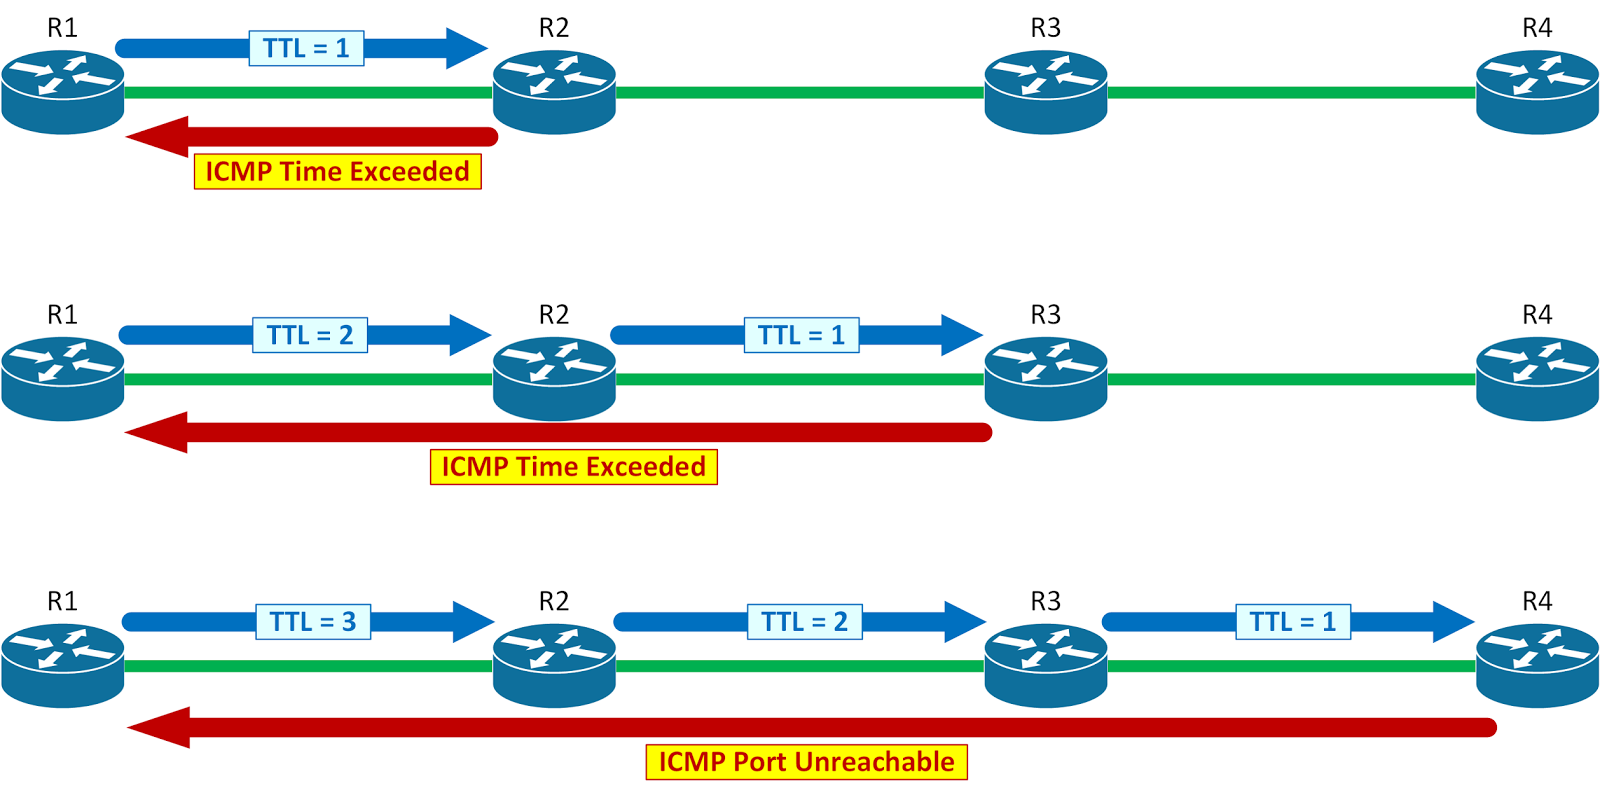
\includegraphics[width=\textwidth]{Imagenes/explicacion_traceroute.png}
  \end{subfigure}
  \label{fig:explicacion_traceroute}
  \caption{Ejemplo de ejecución de nuestro algoritmo para detectar la ruta desde R1 hasta R4}
\end{figure}
\par Nos proponemos analizar los caminos por los cuales distintos paquetes llegan al destino. Para esto usaremos mensajes de protocolo ICMP, donde iremos aumentando el campo \textit{ttl} y provocaremos así que los nodos nos contesten con mensajes del tipo \textit{time exceded}. Controlaremos el tiempo que tarda cada nodo en contestar (\textit{rtt}) por si un hop no responde y luego analizaremos esos valores en busca de saltos intercontinentales.

\par Para determinar si un salto entre dos nodos es intercontinental nos basaremos en la técnica de estimación de outliers propuesta por Cimbala\footnote{http://www.mne.psu.edu/cimbala/me345/Lectures/Outliers.pdf}. Identificaremos outliers y trabajaremos con ellos para determinar si son saltos intercontinentales.
Cimbala propone una métrica basada en un z-score para cada uno de los RTT promedio de cada uno de los hops, el cual está definido de la siguiente manera:

\begin{equation}
    ZRTT_i = \frac{RTT_i-mean(RTT)}{std(RTT)}
\end{equation}
donde $mean(RTT)$ es la media aritmética de los RTTs de la ruta y $std(RTT)$ el desvío estándar.
Luego al mayor de estos valores se lo debe comparar con un valor crítico dado por la siguiente ecuación:

\begin{equation}
    \tau = \frac{t_{\alpha/2}*(n-1)}{\sqrt{n}*\sqrt{n-2+t_{\alpha/2}^{2}}}
\end{equation}
donde $n$ es la cantidad de hops y $t_{\alpha/2}$ es la distribución de student con el parámetro $\alpha=0.05$ y $df =  n-2$
Si $ZRRT_{max} > \tau$ se considera que que esa medición es un outlier y se lo separa de la muestra para luego repetir el proceso desde el cálculo de los ZRTTs
\par Al mismo tiempo, utilizaremos un servicio de api externo\footnote{https://github.com/fiorix/freegeoip} para obtener la geolocalización de cada nodo (por medio de la ip). De esta manera podremos seguir el recorrido del paquete hacia el destino y verificar el funcionamiento del método utilizado para detectar saltos intercontinentales. Para las funciones relativas al manejo de paquetes usamos una biblioteca de Python llamada \emph{Scapy}


\section{Primera captura y análisis}
\par En esta primera instancia vamos a correr nuestra herramienta para un destino en particular y analizaremos los resultados desde dos enfoques. Por una parte, veremos el recorrido de la ruta, los paises por los cuales pasa, el tiempo de respuesta de los distintos nodos y los saltos intercontinentales. Por otro lado, pondremos a prueba el funcionamiento de la herramienta y pensaremos en mejoras o correcciones que creamos pertinentes.

\subsection{Explicación del experimento}
\par Tomaremos como destino el host de la \textbf{Universidad de Ciudad del Cabo [uct.ac.za]}. Como mencionamos previamente, la herramienta irá aumentando el valor del campo \textit{ttl} hasta lograr una respuesta de la ip correspondiente a este host. Enviaremos 50 paquetes por cada valor de ttl, para obtener un buen promedio y evitar casos anormales.

\subsection{Resultados obtenidos}

\begin{figure}[h]
  \begin{subfigure}[b]{.5\textwidth}
    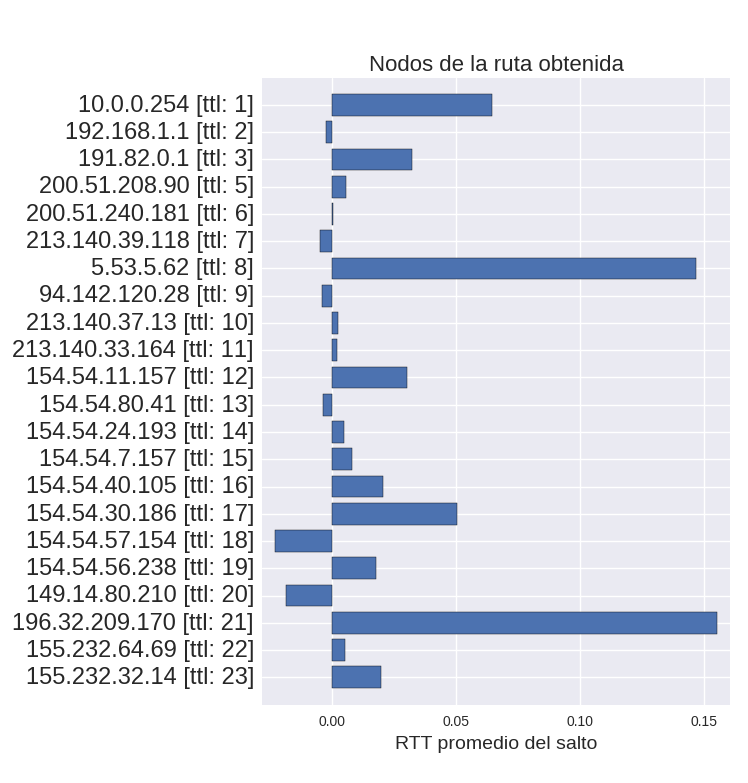
\includegraphics[width=\textwidth]{Imagenes/capetown_rtts.png}
  \end{subfigure}
  \label{fig:capetown_rtts}
  \caption{Tiempo del salto entre cada nodo y su nodo previo, para cada nodo identificado en el camino al host uct.ac.za}
\end{figure}

\begin{figure*}[ht]
  \hspace*{-0.4cm}
  \begin{subfigure}[b]{.60\textwidth}
    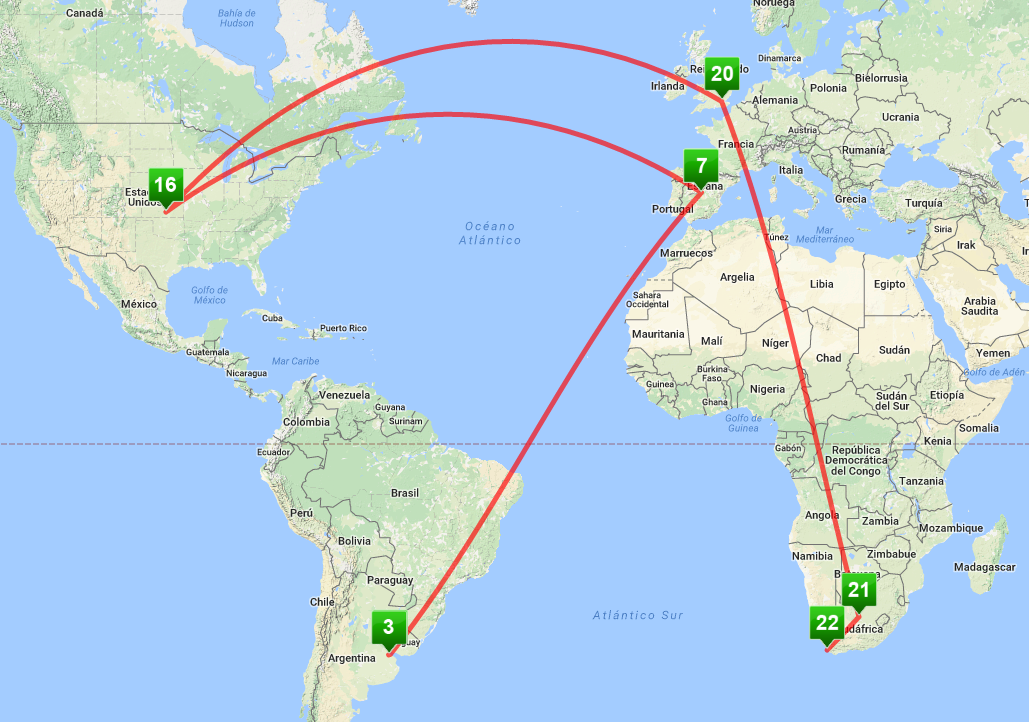
\includegraphics[width=\textwidth]{Imagenes/capetown_map.png}
    \label{fig:capetown_map}
    \caption{Mapa que muestra la unión de los nodos que forman el camino.}
  \end{subfigure}
  \begin{subfigure}[b]{.39\textwidth}
    \footnotesize
    \begin{tabular}{ l l l }
      \hline
      \textbf{TTL} & \textbf{IP} &  \textbf{País - Ciudad} \\ \hline
      1 & 10.0.0.254 &\\ \hline
      2 & 192.168.1.1 &\\ \hline
      \rowcolor[RGB]{196,214,255}
      3 & 191.82.0.1 & Argentina - Libertad\\ \hline
      5 & 200.51.208.90 & Argentina\\ \hline
      6 & 200.51.240.181 & Argentina\\ \hline
      7 & 213.140.39.118 & Spain\\ \hline
      \rowcolor[RGB]{196,214,255}
      8 & 5.53.5.62 & Spain\\ \hline
      9 & 94.142.120.28 & Spain\\ \hline
      10 & 213.140.37.13 & Spain\\ \hline
      11 & 213.140.33.164 & Spain\\ \hline
      \rowcolor[RGB]{196,214,255}
      12 & 154.54.11.157 & United States\\ \hline
      13 & 154.54.80.41 & United States\\ \hline
      14 & 154.54.24.193 & United States\\ \hline
      15 & 154.54.7.157 & United States\\ \hline
      16 & 154.54.40.105 & United States\\ \hline
      \rowcolor[RGB]{196,214,255}
      17 & 154.54.30.186 & United States\\ \hline
      18 & 154.54.57.154 & United States\\ \hline
      19 & 154.54.56.238 & United States\\ \hline
      20 & 149.14.80.210 & United Kingdom - Mayfair\\ \hline
      \rowcolor[RGB]{196,214,255}
      21 & 196.32.209.170 & South Africa\\ \hline
      22 & 155.232.64.69 & South Africa - Wynberg\\ \hline
      23 & 155.232.32.14 & South Africa - Wynberg\\ \hline
      \hline
    \end{tabular}
    \label{fig:capetown_list}
    \caption{Listado de nodos: TTL, IP y país. Se encuentran resaltados los destinos de los saltos intercontinentales.}
  \end{subfigure}
  \caption{Nodos pertenecientes al camino al host uct.ac.za.}
\end{figure*}

\par En la figura 3(a) podemos ver la representación en un planisferio del camino recorrido hacia el destino, junto con la ubicación de los nodos intermedios. Se nota a simple vista lo poco intuitivo que resulta el camino. Pasa por España, Estados Unidos y Reino Unido, para luego llegar a Sudáfrica, donde se redirige a Ciudad del Cabo. Este fué uno de los motivos que nos llevó a elegir este host para ser analizado.

\par En la figura 2 podemos ver el listado de nodos identificados en el camino al host destino y la comparación de los rtt promedio entre cada salto. Para cada nodo, se muestra el tiempo (promediado en segundos) que se tardó en llegar desde el nodo previo hasta él. Este valor se calcula tomando el tiempo que se tardó en llegar al nodo actual y restándole el mismo valor, pero del nodo previo.
\par Podemos ver que algunos valores de RTT resultan negativos. Esto se lo adjudicamos al hecho de que al recibir un paquete con ttl=0 algunos nodos tardan en enviar el paquete de respuesta (\textit{time exceded}), ya sea por restarle prioridad o por algún tema de procesamiento interno. De esta manera, la respuesta del nodo siguiente tal vez tarde menos y nos quede un valor negativo.
\par Otro dato importante que se observa de los resultados es que no se obtuvo respuesta del nodo correspiendiente al ttl=4. Creemos que esto se debe a que algunos nodos se encuentran configurados para no responder mensajes ICMP. En base a esto, tuvimos que tomar la determinación de ignorar los nodos que no respondan y suponer que los nodos previo y posterior se encuentran unidos. Esto influye fuértemente en el cálculo del tiempo de los saltos entre los nodos, ya que algunos saltos contienen en verdad algún nodo interno, el cual puede agregar tiempo.
\par Con los valores de RTT obtenidos, se ejecutó un algoritmo basado en la técnica de estimación de outliers propuesta por John Cimbala\footnote{Outliers - John Cimbala: http://www.mne.psu.edu/cimbala/me345/Lectures/Outliers.pdf} para tratar de predecir saltos intercontinentales. En nuestro caso, solo nos interesan los outliers superiores (con mayor RTT), por lo que nuestro único candidato será el salto con mayor tiempo. El algoritmo se aplicó iterativamente hasta que se concluye que no hay mas outliers, según el criterio mencionado por John Cimbala. De esta manera, en la figura 3(b) se pueden observar los 5 outliers obtenidos por el algoritmo (resaltados en azul), dos de los cuales se corresponden a un salto intercontinental: \textit{España - Estados Unidos} y \textit{Reino Unido - Sudafrica}. Los otros 3 outliers detectados no se corresponden con saltos intercontinentales, pero si observamos el gráfico de la figura 2 podemos corroborar a simple vista que son claramente valores por fuera de lo normal. Volviendo al listado de nodos, vemos que hay 2 saltos intercontinentales que no fueron detectados: \textit{Argentina - España} y \textit{Estados Unidos - Reino Unido}.
\par Podemos concluir que al momento de detectar outliers experimentamos 2 falsos negativos y 3 falsos positivos sobre 5 resultados obtenidos.


\section{Segunda captura y análisis}

\subsection{Explicación del experimento}
\par En este segundo experimento vamos a analizar la ruta desde GBA hasta la \textbf{University of Technology [utech.edu.jm]}, ubicada en Kingston, Jamaica. Dado que Jamaica es una isla, la ruta debe tener al menos un salto por agua.

\subsection{Resultados obtenidos}

\begin{figure}[h!]
  \begin{subfigure}[b]{.5\textwidth}
    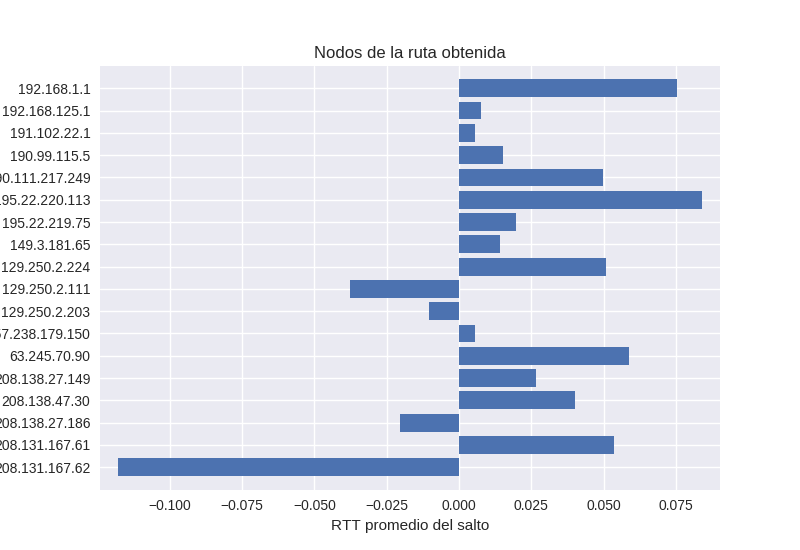
\includegraphics[width=\textwidth]{Imagenes/jamaica_rtts.png}
  \end{subfigure}
  \label{fig:jamaica_rtts}
  \caption{Tiempo del salto entre cada nodo y su nodo previo, para cada nodo identificado en el camino al host utech.edu.jm}
\end{figure}

\par En el gráfico correspondiente a la figura 4 se puede observar que los promedios positivos no varían mucho, en particular la media muestral de todos los datos (negativos o positivos) es 0.025796904867776 mientras que la varianza es 0.001129809044593, que son algunos órdenes de magnitud menos. Que la varianza sea tan pequeña nos quiere decir que los datos no presentan una gran dispersión y, por ende, no es muy probable que haya outliers.

\begin{figure}[h!]
  \begin{subfigure}[b]{.5\textwidth}
    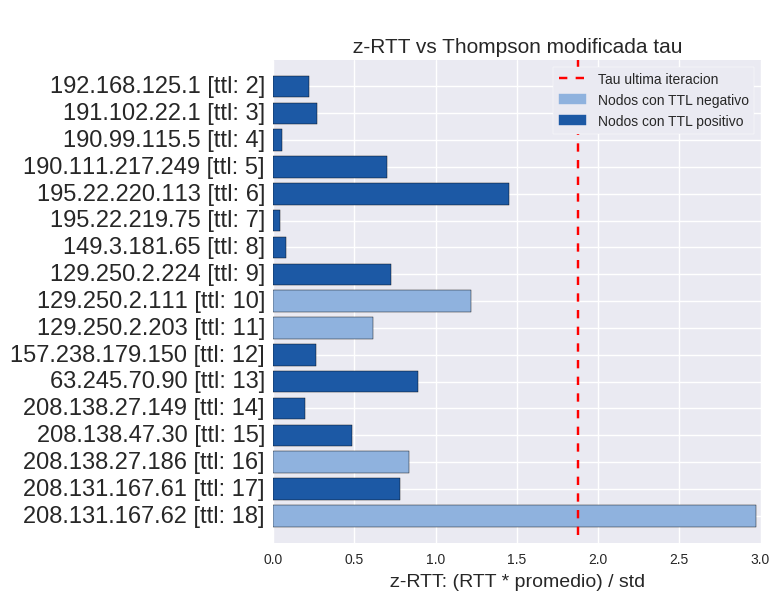
\includegraphics[width=\textwidth]{Imagenes/jamaica_zrtts.png}
  \end{subfigure}
  \label{fig:jamaica_zrtts}
  \caption{zRTT de los nodos del camino al host utech.edu.jm comparado con el umbral establecido por el valor de Thompson modificado.}
\end{figure}

\begin{figure*}[ht]
  \hspace*{-0.4cm}
  \begin{subfigure}[b]{.60\textwidth}
    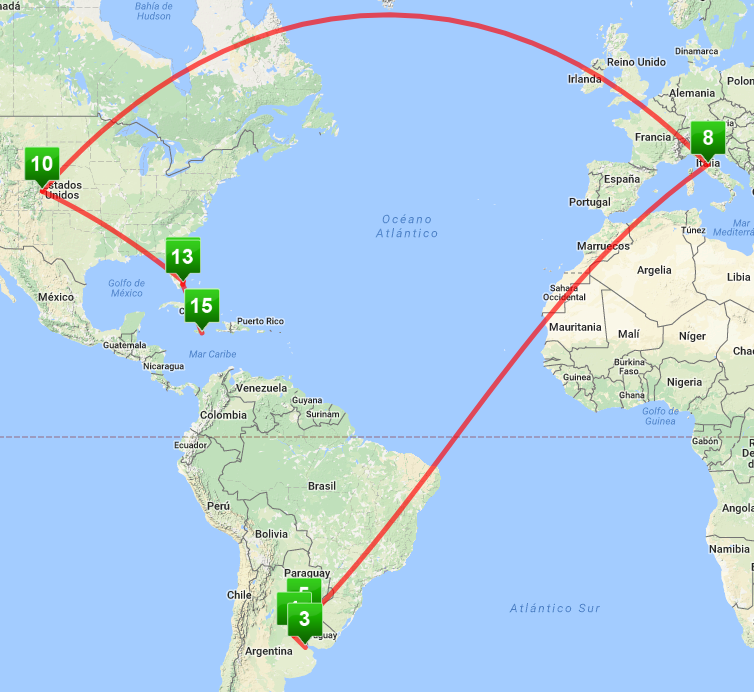
\includegraphics[width=\textwidth]{Imagenes/jamaica_map.png}
    \label{fig:jamaica_map}
    \caption{Mapa que muestra la unión de los nodos que forman el camino.}
  \end{subfigure}
  \begin{subfigure}[b]{.39\textwidth}
    \footnotesize
    \begin{tabular}{ l l l }
      \hline
      \textbf{TTL} & \textbf{IP} &  \textbf{País - Ciudad} \\ \hline
      1 & 192.168.1.1 &\\ \hline
      2 & 192.168.125.1 &\\ \hline
      3 & 191.102.22.1 & Argentina - Morón\\ \hline
      4 & 190.99.115.5 & Argentina - Rosario\\ \hline
      5 & 190.111.217.249 & Argentina - Entre Ríos\\ \hline
      \rowcolor[RGB]{196,214,255}
      6 & 195.22.220.113 & Italia\\ \hline
      7 & 195.22.219.75 & Italia\\ \hline
      8 & 149.3.181.65 & Italia\\ \hline
      \rowcolor[RGB]{196,214,255}
      9 & 129.250.2.224 & Estados Unidos - Colorado \\ \hline
      10 & 129.250.2.111 & Estados Unidos - Colorado\\ \hline
      11 & 129.250.2.203 & Estados Unidos - Colorado\\ \hline
      12 & 157.238.179.150 & Estados Unidos - Florida\\ \hline
      13 & 63.245.70.90 & Estados Unidos - Florida\\ \hline
      \rowcolor[RGB]{196,214,255}
      14 & 208.138.27.149 & Jamaica - Kinsgton\\ \hline
      15 & 208.138.47.30 & Jamaica - Kingston\\ \hline
      16 & 208.138.27.186 & Jamaica - Kingston\\ \hline
      17 & 208.131.167.61 & Jamaica - Kingston\\ \hline
      18 & 208.131.167.62 & Jamaica - Kingston \\ \hline
      \hline
    \end{tabular}
    \label{fig:jamaica_list}
    \caption{Listado de nodos: TTL, IP y ubicación geográfica.}
  \end{subfigure}
  \caption{Nodos pertenecientes al camino al host utech.edu.jm.}
\end{figure*}

\par Luego, ejecutamos nuestro algoritmo de detección de outliers y, como era de esperar, no se obtuvieron outliers. En la tabla en la que exhibimos la ruta se muestran en azul los tres saltos intercontinentales que realizaron los paquetes hasta llegar a la University of Technology. Esto es particularmente llamativo dado que según el planisferio de enlaces intercontinentales\footnote{Mapa de enlaces intercontinentales: http://www.muycomputer.com/wp-content/uploads/2011/09/mundo.86i.cyp3mivcag.jpeg} hay por lo menos dos caminos posibles cuya longitud es mucho menor (un enlace desde Chile hasta Panamá y luego desde Panamá hasta Jamaica y la otra opción es ir por la costa de Brasil para luego acceder a Jamaica). La explicación que le pudimos encontrar a este comportamiento es que al haber muchísimos enlaces entre Europa y Estados Unidos la red prefiere ir hacia Europa para luego tener varias opciones para regresar al continente americano.
\par En este caso todos los hops respondieron nuestros mensajes. La ruta, a nuestro criterio, no es tan larga, pero tiene demasiados saltos intercontinentales.


\section{Tercera captura y análisis}

\subsection{Explicación del experimento}
\par En este tercer experimento vamos a analizar la ruta desde GBA hasta la \textbf{Universidad de Abai [kaznpu.kz]}, ubicada en Almatý, Kazajistán. Kazajistán está ubicado en el centro de Asia y sólo tiene costa en el mar Caspio, por lo que cualquier paquete que desee acceder a dicho país debe pasar primero por una nación que tenga salida al océano.

\subsection{Resultados obtenidos}

\begin{figure}[h!]
  \begin{subfigure}[b]{.5\textwidth}
    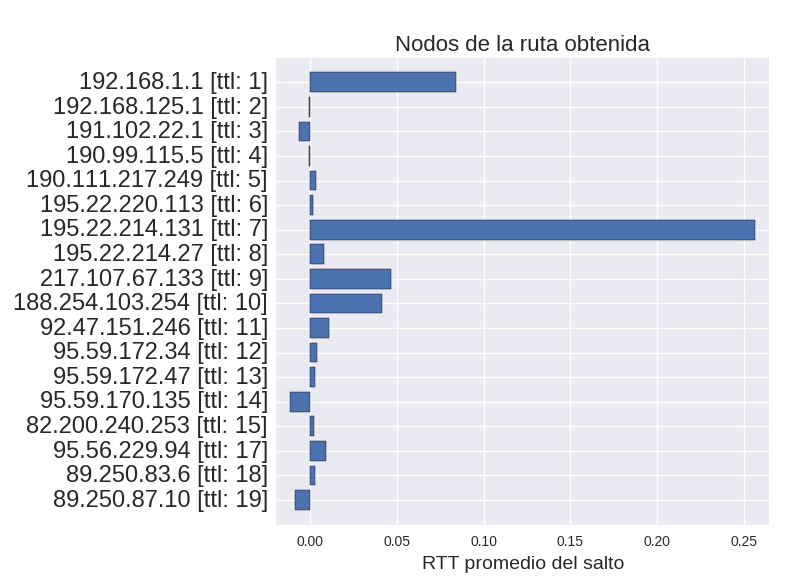
\includegraphics[width=\textwidth]{Imagenes/kazajistan_rtts.png}
  \end{subfigure}
  \label{fig:kazajthan_rtts}
  \caption{Tiempo del salto entre cada nodo y su nodo previo, para cada nodo identificado en el camino al host kaznpu.kz}
\end{figure}

\begin{figure*}[ht]
  \hspace*{-0.4cm}
  \begin{subfigure}[b]{.60\textwidth}
    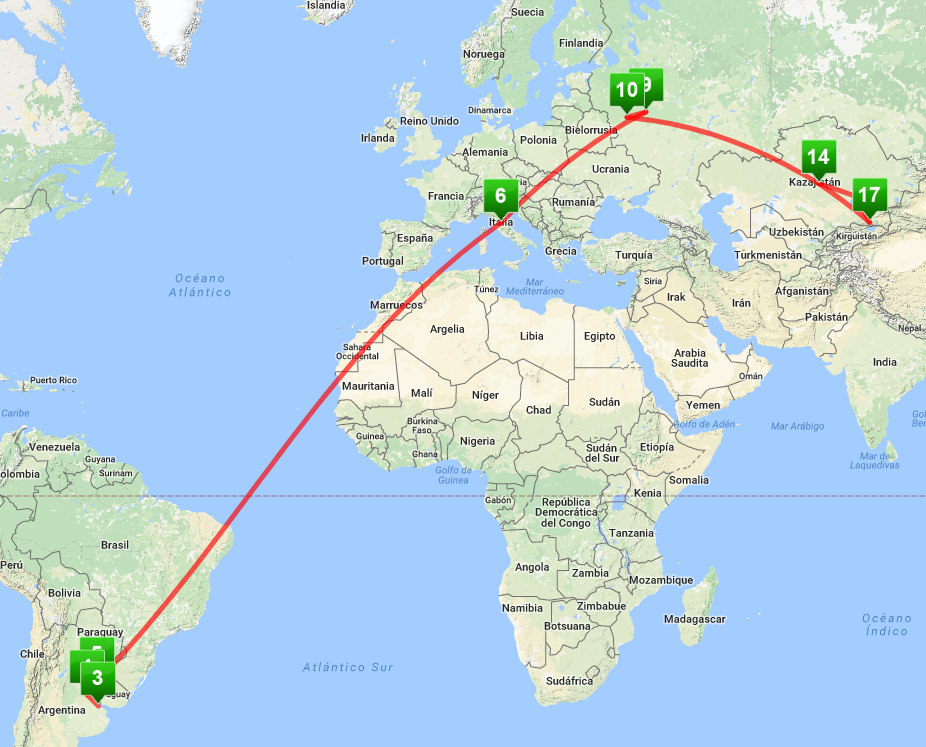
\includegraphics[width=\textwidth]{Imagenes/kazajistan_map.png}
    \label{fig:kazajthan_map}
    \caption{Mapa que muestra la unión de los nodos que forman el camino.}
  \end{subfigure}
  \begin{subfigure}[b]{.39\textwidth}
    \footnotesize
    \begin{tabular}{ l l l }
      \hline
      \textbf{TTL} & \textbf{IP} &  \textbf{País - Ciudad} \\ \hline
      1 & 192.168.1.1 &\\ \hline
      2 & 192.168.125.1 &\\ \hline
      3 & 191.102.22.1 & Argentina - Morón\\ \hline
      4 & 190.99.115.5 & Argentina - Rosario\\ \hline
      5 & 190.111.217.249 & Argentina - Entre Ríos\\ \hline
      6 & 195.22.220.113 & Italia\\ \hline
      \rowcolor[RGB]{196,214,255}
      7 & 195.22.214.131 & Italia\\ \hline
      8 & 195.22.214.27 & Italia\\ \hline
      \rowcolor[RGB]{196,214,255}
      9 & 217.107.67.133 & Rusia - Moscú \\ \hline
      \rowcolor[RGB]{196,214,255}
      10 & 188.254.103.254 & Rusia - Smolenskaya Oblast\\ \hline
      11 & 92.47.151.246 & Kazajthan\\ \hline
      12 & 95.59.172.34 & Kazajthan\\ \hline
      13 & 95.59.172.47 & Kazajthan\\ \hline
      14 & 95.59.170.135 & Kazajthan\\ \hline
      15 & 82.200.240.253 & Kazajthan\\ \hline
      17 & 95.56.229.94 & Kazajthan - Almaty Qalasy\\ \hline
      18 & 89.250.83.6 & Kazajthan\\ \hline
      19 & 89.250.87.10 & Kazajthan\\ \hline
      \hline
    \end{tabular}
    \label{fig:kazajthan_list}
    \caption{Listado de nodos: TTL, IP y ubicación geográfica.}
  \end{subfigure}
  \caption{Nodos pertenecientes al camino al host kaznpu.kz.}
\end{figure*}

\par En el gráfico de la figura 7 se observa un pico muy alto para llegar al hop cuya dirección IP es 195.22.214.131. Esto es bastante extraño porque su recorrido es local, suponemos que la causa de este comportamiento anómalo se debe a que en el hop de llegada había mucha congestión.
\par En el gráfico de la figura 9 podemos ver los 3 nodos que superan la linea del valor de Thompson. Estos son nuestros 3 outliers y candidatos a saltos intercontinentales, según nuestra herramienta. Pero como vemos en la tabla de la figura 8(b), ninguno de los 3 corresponden a saltos intercontinentales. Pero si notamos algo raro en la ruta: de \textit{Kazajthan} se redirecciona a \textit{Kazajthan - Almaty Qalasy} para luego volver a \textit{Kazajthan} inmediatamente. Notamos también que el salto de ida (hacia \textit{Almaty Qalasy}) trae aparejado un rtt un mucho mas elevado que el salto del regreso. No creemos saber por qué puede estar sucediendo esto, pero es un dato interesante que valía mencionar.

\begin{figure}[h]
  \begin{subfigure}[b]{.5\textwidth}
    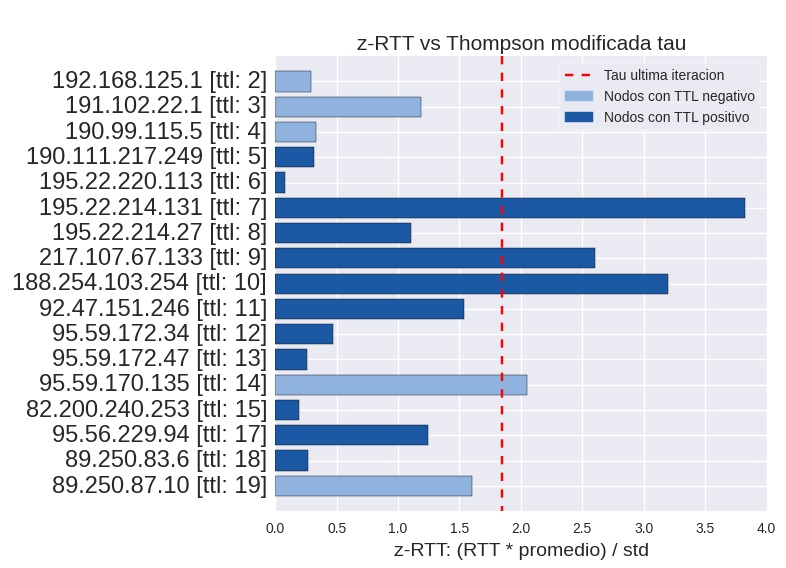
\includegraphics[width=\textwidth]{Imagenes/kazajistan_zrtts.png}
  \end{subfigure}
  \label{fig:kazajthan_zrtts}
  \caption{zRTT de los nodos del camino al host kaznpu.kz comparado con el umbral establecido por el valor de Thompson modificado.}
\end{figure}

\par Con respecto a los saltos intercontinentales, sólo hubo uno y nuestro algoritmo no logró detectarlo. A comparación de los otros experimentos la ruta final es bastante intuitiva, ya que resulta similar al camino óptimo en cuanto a recorrido (una línea recta). Al salir del país pasa por Italia, luego por Rusia y termina en la universidad de destino. Nuevamente, la mayoría de los hops respondió nuestros mensajes, lo cual permitió conocer mejor el trayecto.


\section{Conclusiones}
\par En el siguiente documento \footnote{http://www.net.in.tum.de/fileadmin/TUM/NET/NET-2012-08-1/NET-2012-08-1_02.pdf} Martin Jobst plantea varios casos de comportamientos anómalos en los traceroutes que uno puede llegar a obtener. En nuestros experimentos nos hemos encontrado con varios de ellos, por ejemplo en los traceroutes a Ciudad del cabo y a Kazajthan hubo algunos hops que no respondieron. Aún así este error no impactó en el análisis que realizamos ya que no perdimos ningún salto intercontinental en el medio.
\par También comenta que quien no responde nuestros mensajes puede ser el último nodo de nuestro camino, es decir el destino de nuestra ruta. Este problema lo hemos tenido en algunas universidades con las cuales habíamos experimentado, pero como la mayor parte de los hops de su traceroute tampoco habían respondido no teníamos material suficiente para analizar la ruta. En particular, las universidades que no nos respondieron están ubicadas en China y en Corea del Norte.
\par Por último, otro problema que tuvimos en los tres experimentos fue que el RTT que nos reportaba era falso, en particular porque el RTT hasta algunos hops era menor que el de su predecesor, Jobst comenta que una causa posible de esta anomalía es que las tablas de ruteo generan que el camino de regreso no sea el mismo que el de partida. El caso más problemático fue el traceroute a Jamaica, que creemos que desde su último hop se genera una ruta más directa hacia Argentina. \\
\par Por otro lado, por la naturaleza del método de Cimbala, se espera que la cantidad de saltos intercontinentales sea despreciable frente a la cantidad de saltos a hops cercanos. De esta manera si para llegar a destino hay que realizar varios saltos intercontinentales (como el caso del segundo experimento) y no hay un gran recorrido intracontinental para compensar no se van a poder detectar los saltos intercontinentales.
\par También pensamos la posibilidad de generar un valor de corte fijo para ZRTT y creemos que de esa manera no se puede subsanar la falla que posee ese método. Aún así las predicciones del método de Cimbala en casos normales predice con muy buena exactitud.




\end{document}
